\documentclass[11pt,a4paper]{jsarticle}

\usepackage{amsmath,amssymb}
\usepackage{bm}
\usepackage{graphicx}
\usepackage{ascmac}
\usepackage{subfigure}
\newlength{\subfigwidth}
\newlength{\subfigcolsep}

\graphicspath{{./img/}}

\title{TPC-H performance measure}
\author{Keisuke Suzuki}

\begin{document}
\maketitle
\section{実験環境}
\begin{itemize}
 \item CPU : Xeon X7560 @ 2.27GHz x4
 \item Memory : 64GB
 \item DBMS : PostgreSQL 9.2
 \item RAID0 : iodrive x8 (chunk size = 64KB)
 \item 各テーブルのprimary key上にB-tree indexを構築
 \item Scale Factor = 100
 \item shared buffer = 8GB
 \item 各クエリの実行時の状況をiostatとmpstatで1秒おきに監視
\end{itemize}

\section{Query 1 by index scan on l\_shipdate}
\subsection{microbenchmark}
microbenchで計測したIOの性能がread-aheadの有無やO\_DIRECTの有無に
よって、乱れる場合があった。
乱れの原因となっている部分を確認するため、以下のパラメタを変化させて挙動
を観察する。(iosize = 8KB)

パラメタ
\begin{itemize}
 \item read-ahead: 0 or 2048
 \item O\_DIRECT: 有 or 無
 \item iodrive単体 or raid0
\end{itemize}

\clearpage
\subsubsection{random read microbenchmark結果}
\begin{figure}[thbp]
 \setlength{\subfigwidth}{.5\linewidth}
 \addtolength{\subfigwidth}{-.5\subfigcolsep}
 \begin{minipage}[b]{\subfigwidth}
  \subfigure[IOPS]{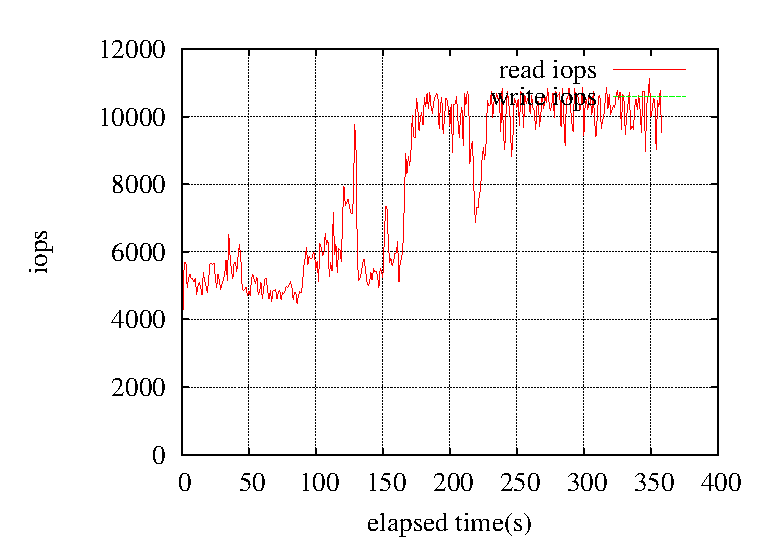
\includegraphics[width=75mm]{md0_rand_8k_ra0iops.eps}
  \label{fig:md0rand8k0iops}}
 \end{minipage}
  \begin{minipage}[b]{\subfigwidth}
   \subfigure[iosize]{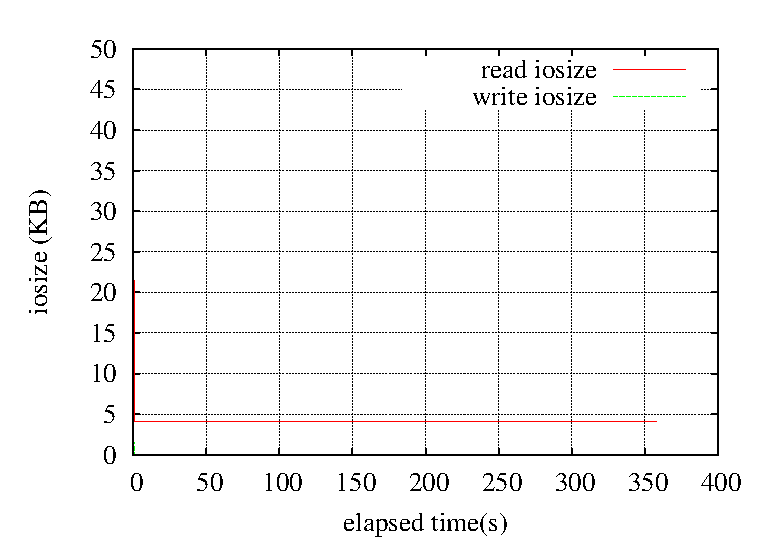
\includegraphics[width=75mm]{md0_rand_8k_ra0iosize.eps}
   \label{fig:md0rand8k0iosize}}
  \end{minipage}
  \caption{read-ahead = 0, w/o O\_DIRECT, raid0}
  \label{fig:md0rand8k0}
\end{figure}

\begin{figure}[thbp]
 \setlength{\subfigwidth}{.5\linewidth}
 \addtolength{\subfigwidth}{-.5\subfigcolsep}
 \begin{minipage}[b]{\subfigwidth}
  \subfigure[IOPS]{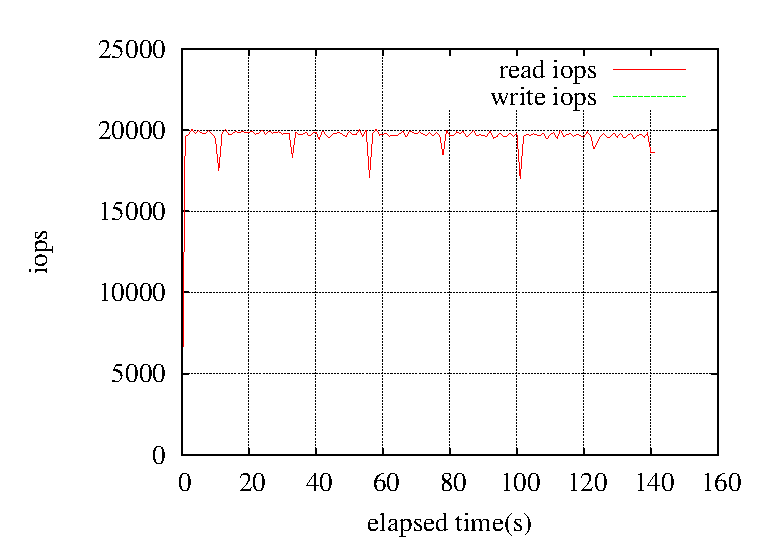
\includegraphics[width=75mm]{fioa_rand_8k_ra0iops.eps}
  \label{fig:fioarand8k0iops}}
 \end{minipage}
  \begin{minipage}[b]{\subfigwidth}
    \subfigure[iosize]{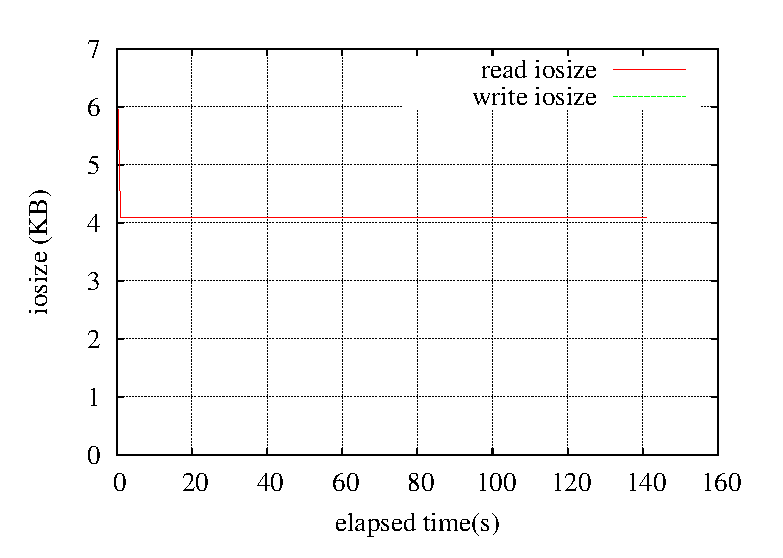
\includegraphics[width=75mm]{fioa_rand_8k_ra0iosize.eps}
   \label{fig:fioarand8k0iosize}}
  \end{minipage}
  \caption{read-ahead = 0, w/o O\_DIRECT, standalone}
  \label{fig:fioarand8k0}
\end{figure}

図\ref{fig:md0rand8k0iops}では、性能が大きく乱れており、同じ計測を繰り
返すと毎回異なるグラフになっていて、実行時間も大きく変化していた。
iodrive単体の上での計測ではこのような結果にはならなかったので、
software raidの部分に原因があると想定される。

\clearpage
\begin{figure}[thbp]
 \setlength{\subfigwidth}{.5\linewidth}
 \addtolength{\subfigwidth}{-.5\subfigcolsep}
 \begin{minipage}[b]{\subfigwidth}
  \subfigure[IOPS]{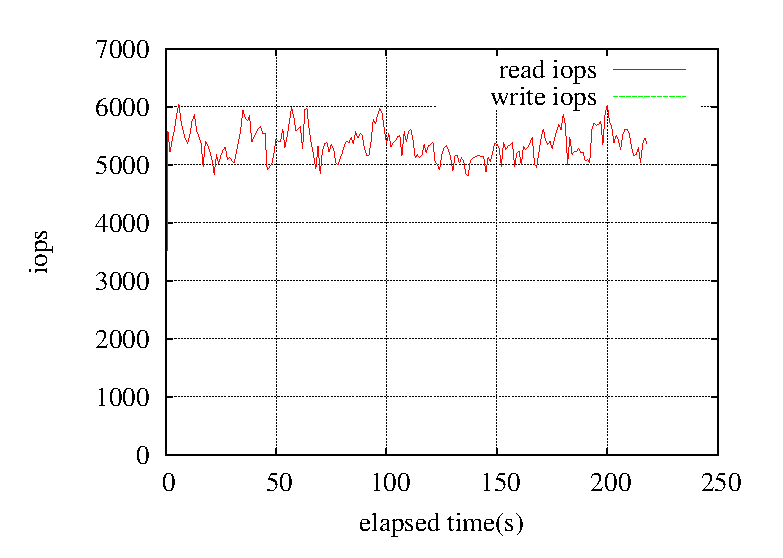
\includegraphics[width=75mm]{md0_rand_8k_ra0_woodirectiops.eps}
  \label{fig:md0rand8k0wodiops}}
 \end{minipage}
  \begin{minipage}[b]{\subfigwidth}
    \subfigure[iosize]{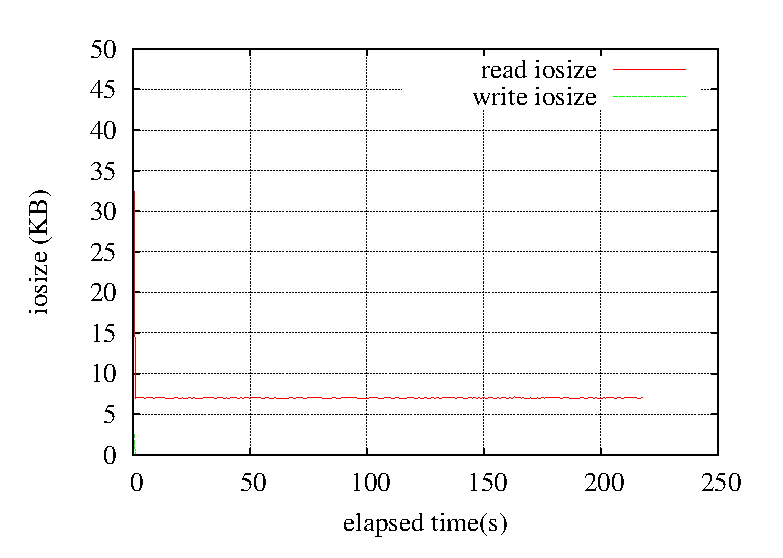
\includegraphics[width=75mm]{md0_rand_8k_ra0_woodirectiosize.eps}
   \label{fig:md0rand8k0wodiosize}}
  \end{minipage}
  \caption{read-ahead = 0, w/ O\_DIRECT, raid0}
  \label{fig:md0rand8k0wod}
\end{figure}

\begin{figure}[thbp]
 \setlength{\subfigwidth}{.5\linewidth}
 \addtolength{\subfigwidth}{-.5\subfigcolsep}
 \begin{minipage}[b]{\subfigwidth}
  \subfigure[IOPS]{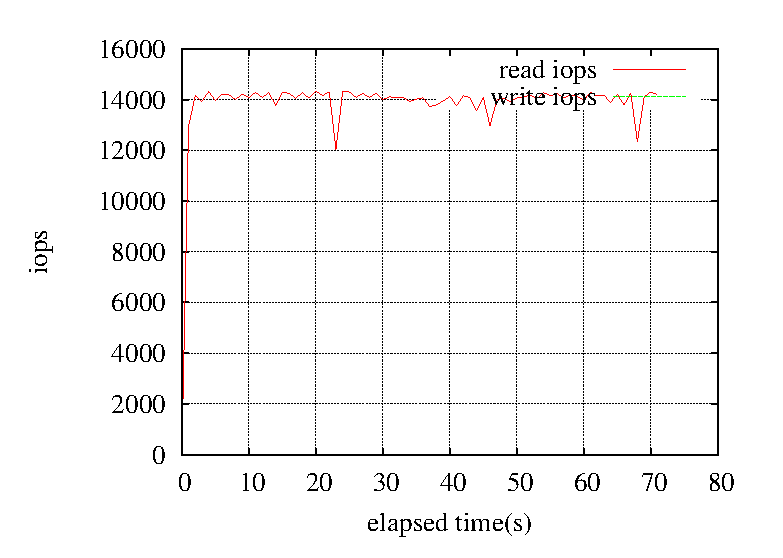
\includegraphics[width=75mm]{fioa_rand_8k_ra0_wodirectiops.eps}
  \label{fig:fioarand8k0wodiops}}
 \end{minipage}
  \begin{minipage}[b]{\subfigwidth}
    \subfigure[iosize]{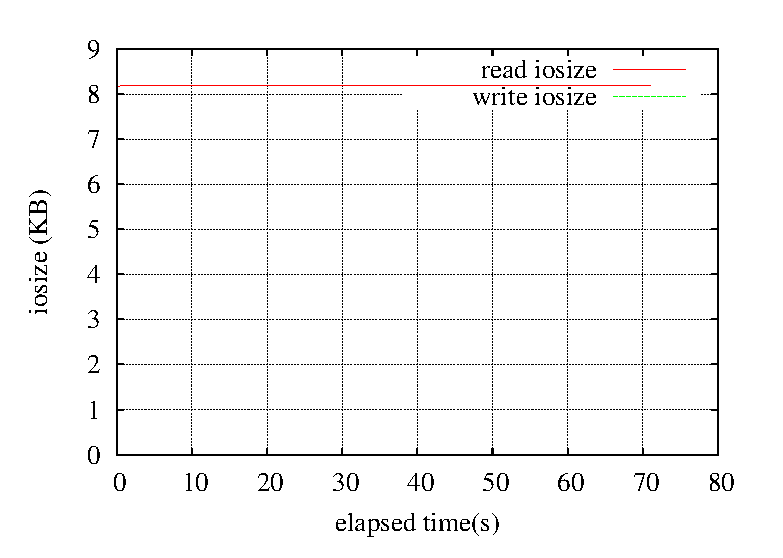
\includegraphics[width=75mm]{fioa_rand_8k_ra0_wodirectiosize.eps}
   \label{fig:fioarand8k0wodiosize}}
  \end{minipage}
  \caption{read-ahead = 0, w/ O\_DIRECT, standalone}
  \label{fig:fioarand8k0wod}
\end{figure}

\clearpage
\begin{figure}[thbp]
 \setlength{\subfigwidth}{.5\linewidth}
 \addtolength{\subfigwidth}{-.5\subfigcolsep}
 \begin{minipage}[b]{\subfigwidth}
  \subfigure[IOPS]{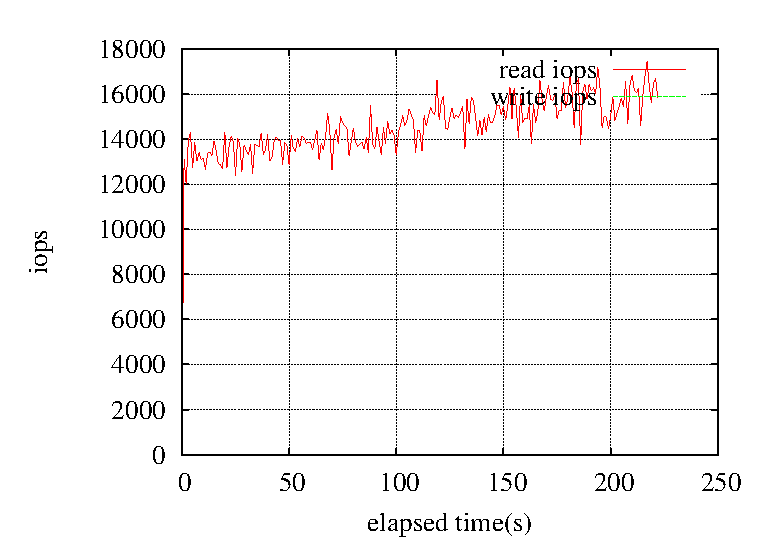
\includegraphics[width=75mm]{md0_rand_8k_ra2048iops.eps}
  \label{fig:md0rand8k2048iops}}
 \end{minipage}
  \begin{minipage}[b]{\subfigwidth}
    \subfigure[iosize]{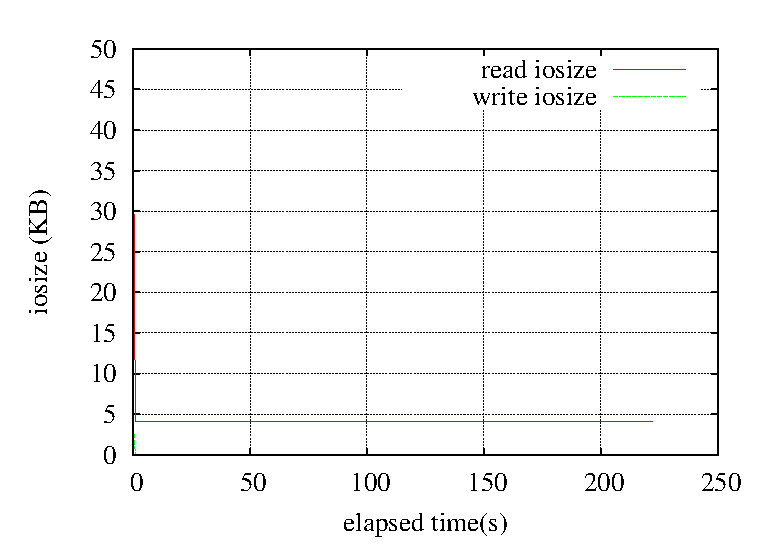
\includegraphics[width=75mm]{md0_rand_8k_ra2048iosize.eps}
   \label{fig:md0rand8k2048iosize}}
  \end{minipage}
  \caption{read-ahead = 2048, w/o O\_DIRECT, raid0}
  \label{fig:md0rand8k2048}
\end{figure}

\begin{figure}[thbp]
 \setlength{\subfigwidth}{.5\linewidth}
 \addtolength{\subfigwidth}{-.5\subfigcolsep}
 \begin{minipage}[b]{\subfigwidth}
  \subfigure[IOPS]{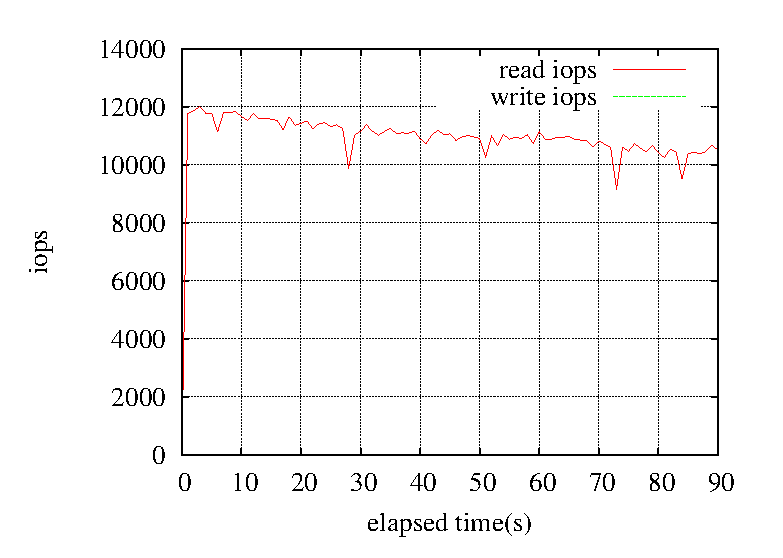
\includegraphics[width=75mm]{fioa_rand_8k_ra256iops.eps}
  \label{fig:fioarand8k256iops}}
 \end{minipage}
  \begin{minipage}[b]{\subfigwidth}
    \subfigure[iosize]{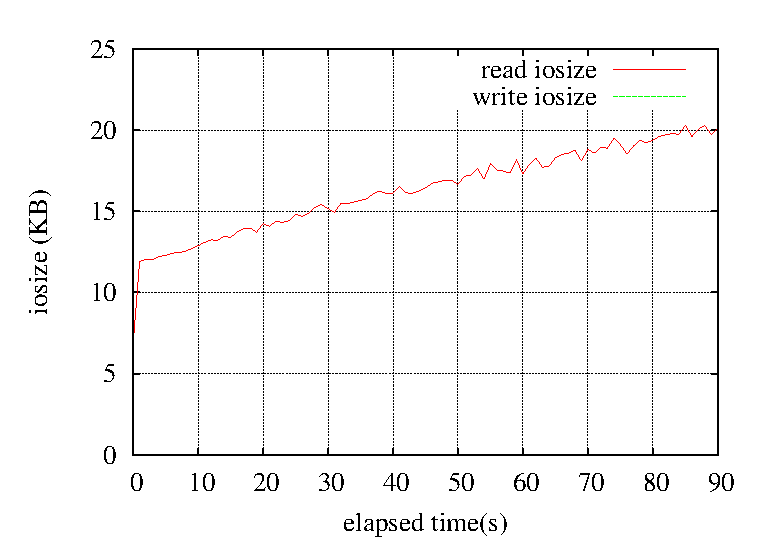
\includegraphics[width=75mm]{fioa_rand_8k_ra256iosize.eps}
   \label{fig:fioarand8k256iosize}}
  \end{minipage}
  \caption{read-ahead = 256, w/o O\_DIRECT, standalone}
  \label{fig:fioarand8k256}
\end{figure}

\clearpage
\begin{figure}[thbp]
 \setlength{\subfigwidth}{.5\linewidth}
 \addtolength{\subfigwidth}{-.5\subfigcolsep}
 \begin{minipage}[b]{\subfigwidth}
  \subfigure[IOPS]{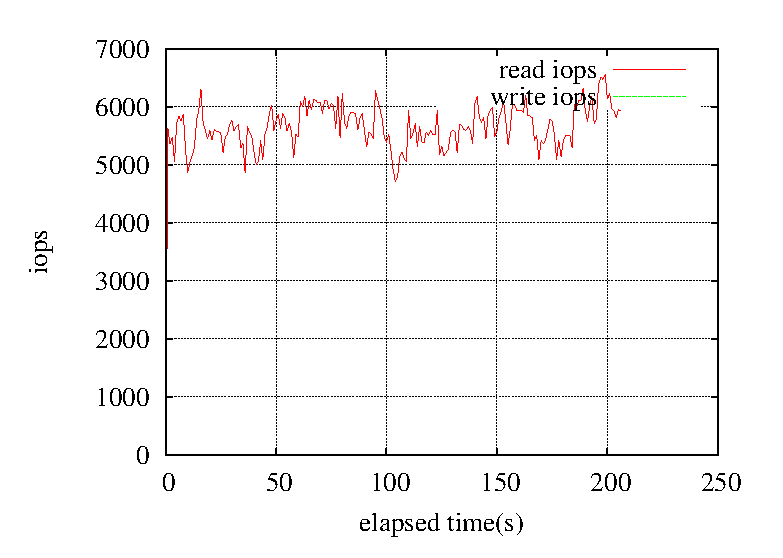
\includegraphics[width=75mm]{md0_rand_8k_ra2048_wodirectiops.eps}
  \label{fig:md0rand8k2048wodiops}}
 \end{minipage}
  \begin{minipage}[b]{\subfigwidth}
    \subfigure[iosize]{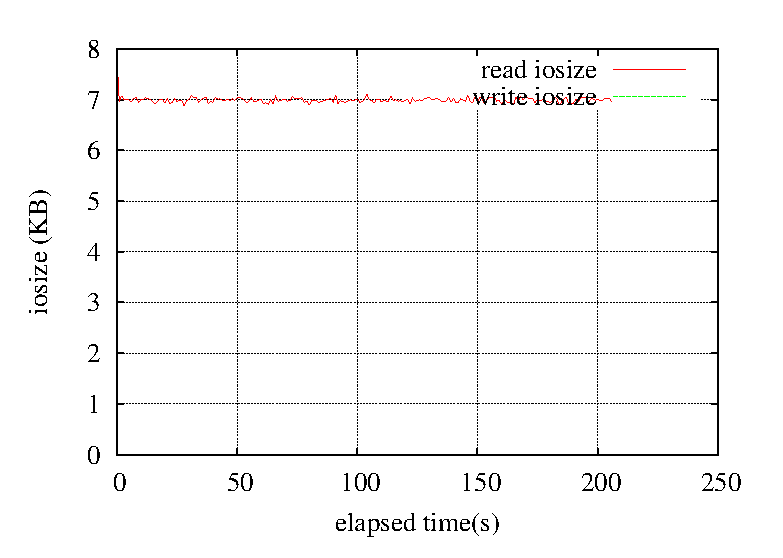
\includegraphics[width=75mm]{md0_rand_8k_ra2048_wodirectiosize.eps}
   \label{fig:md0rand8k2048wodiosize}}
  \end{minipage}
  \caption{read-ahead = 2048, w/ O\_DIRECT, raid0}
  \label{fig:md0rand8k2048wod}
\end{figure}

\begin{figure}[thbp]
 \setlength{\subfigwidth}{.5\linewidth}
 \addtolength{\subfigwidth}{-.5\subfigcolsep}
 \begin{minipage}[b]{\subfigwidth}
  \subfigure[IOPS]{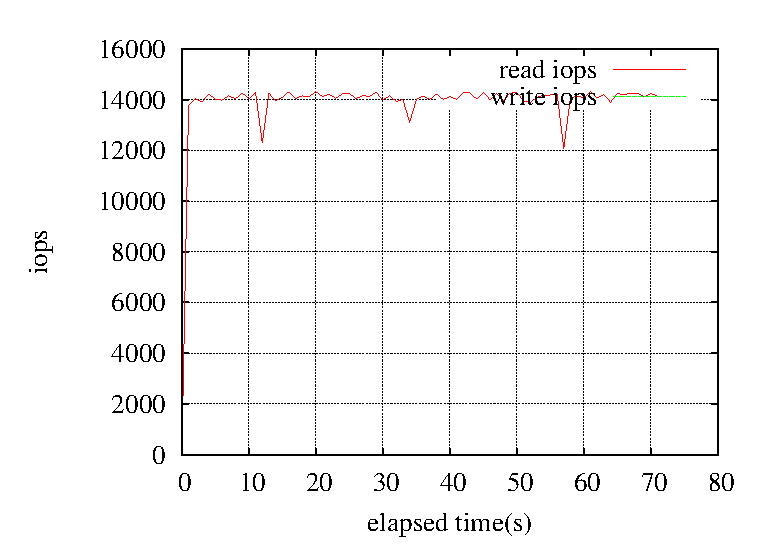
\includegraphics[width=75mm]{fioa_rand_8k_ra256_wodirectiops.eps}
  \label{fig:fioarand8k256wodiops}}
 \end{minipage}
  \begin{minipage}[b]{\subfigwidth}
    \subfigure[iosize]{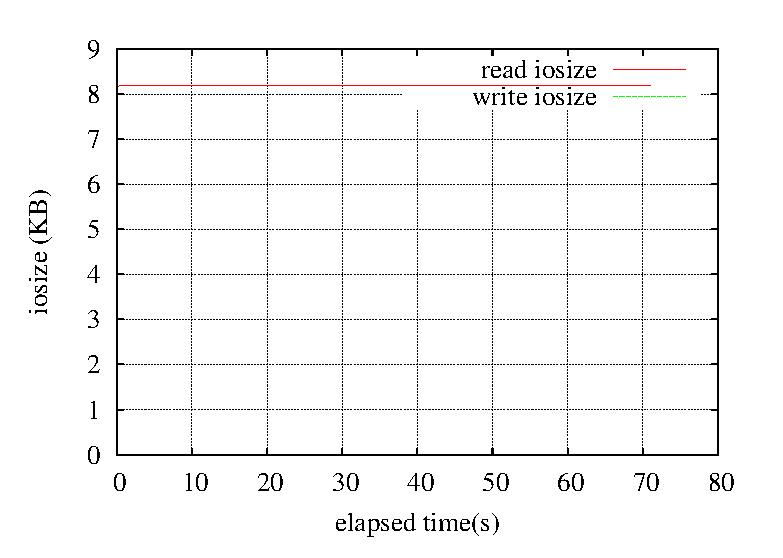
\includegraphics[width=75mm]{fioa_rand_8k_ra256_wodirectiosize.eps}
   \label{fig:fioarand8k256wodiosize}}
  \end{minipage}
  \caption{read-ahead = 256, w/ O\_DIRECT, standalone}
  \label{fig:fioarand8k256wod}
\end{figure}

raidの方では複数のLUにまたがるアドレスへのアクセスが含まれる場合があるた
め、iosizeが8kよりは小くなっている。

\clearpage
\section{Query 8}
簡単の為、Query8のうちのIOがメインとなる部分のみを実行する。

\subsection{Query and Execution Plan}
\begin{verbatim}
 select
	extract(year from o_orderdate) as o_year,
	l_extendedprice * (1 - l_discount) as volume,
	n2.n_name as nation
from
	part, supplier, lineitem, orders,
	customer, nation n1, nation n2,	region
where
	p_partkey = l_partkey
	and s_suppkey = l_suppkey
	and l_orderkey = o_orderkey
	and o_custkey = c_custkey
	and c_nationkey = n1.n_nationkey
	and n1.n_regionkey = r_regionkey
	and r_name = 'AMERICA'
	and s_nationkey = n2.n_nationkey
	and o_orderdate between date '1995-01-01' and date '1996-12-31'
	and p_type = 'ECONOMY ANODIZED STEEL'
\end{verbatim}

\begin{figure}[thbp]
 \begin{center}
  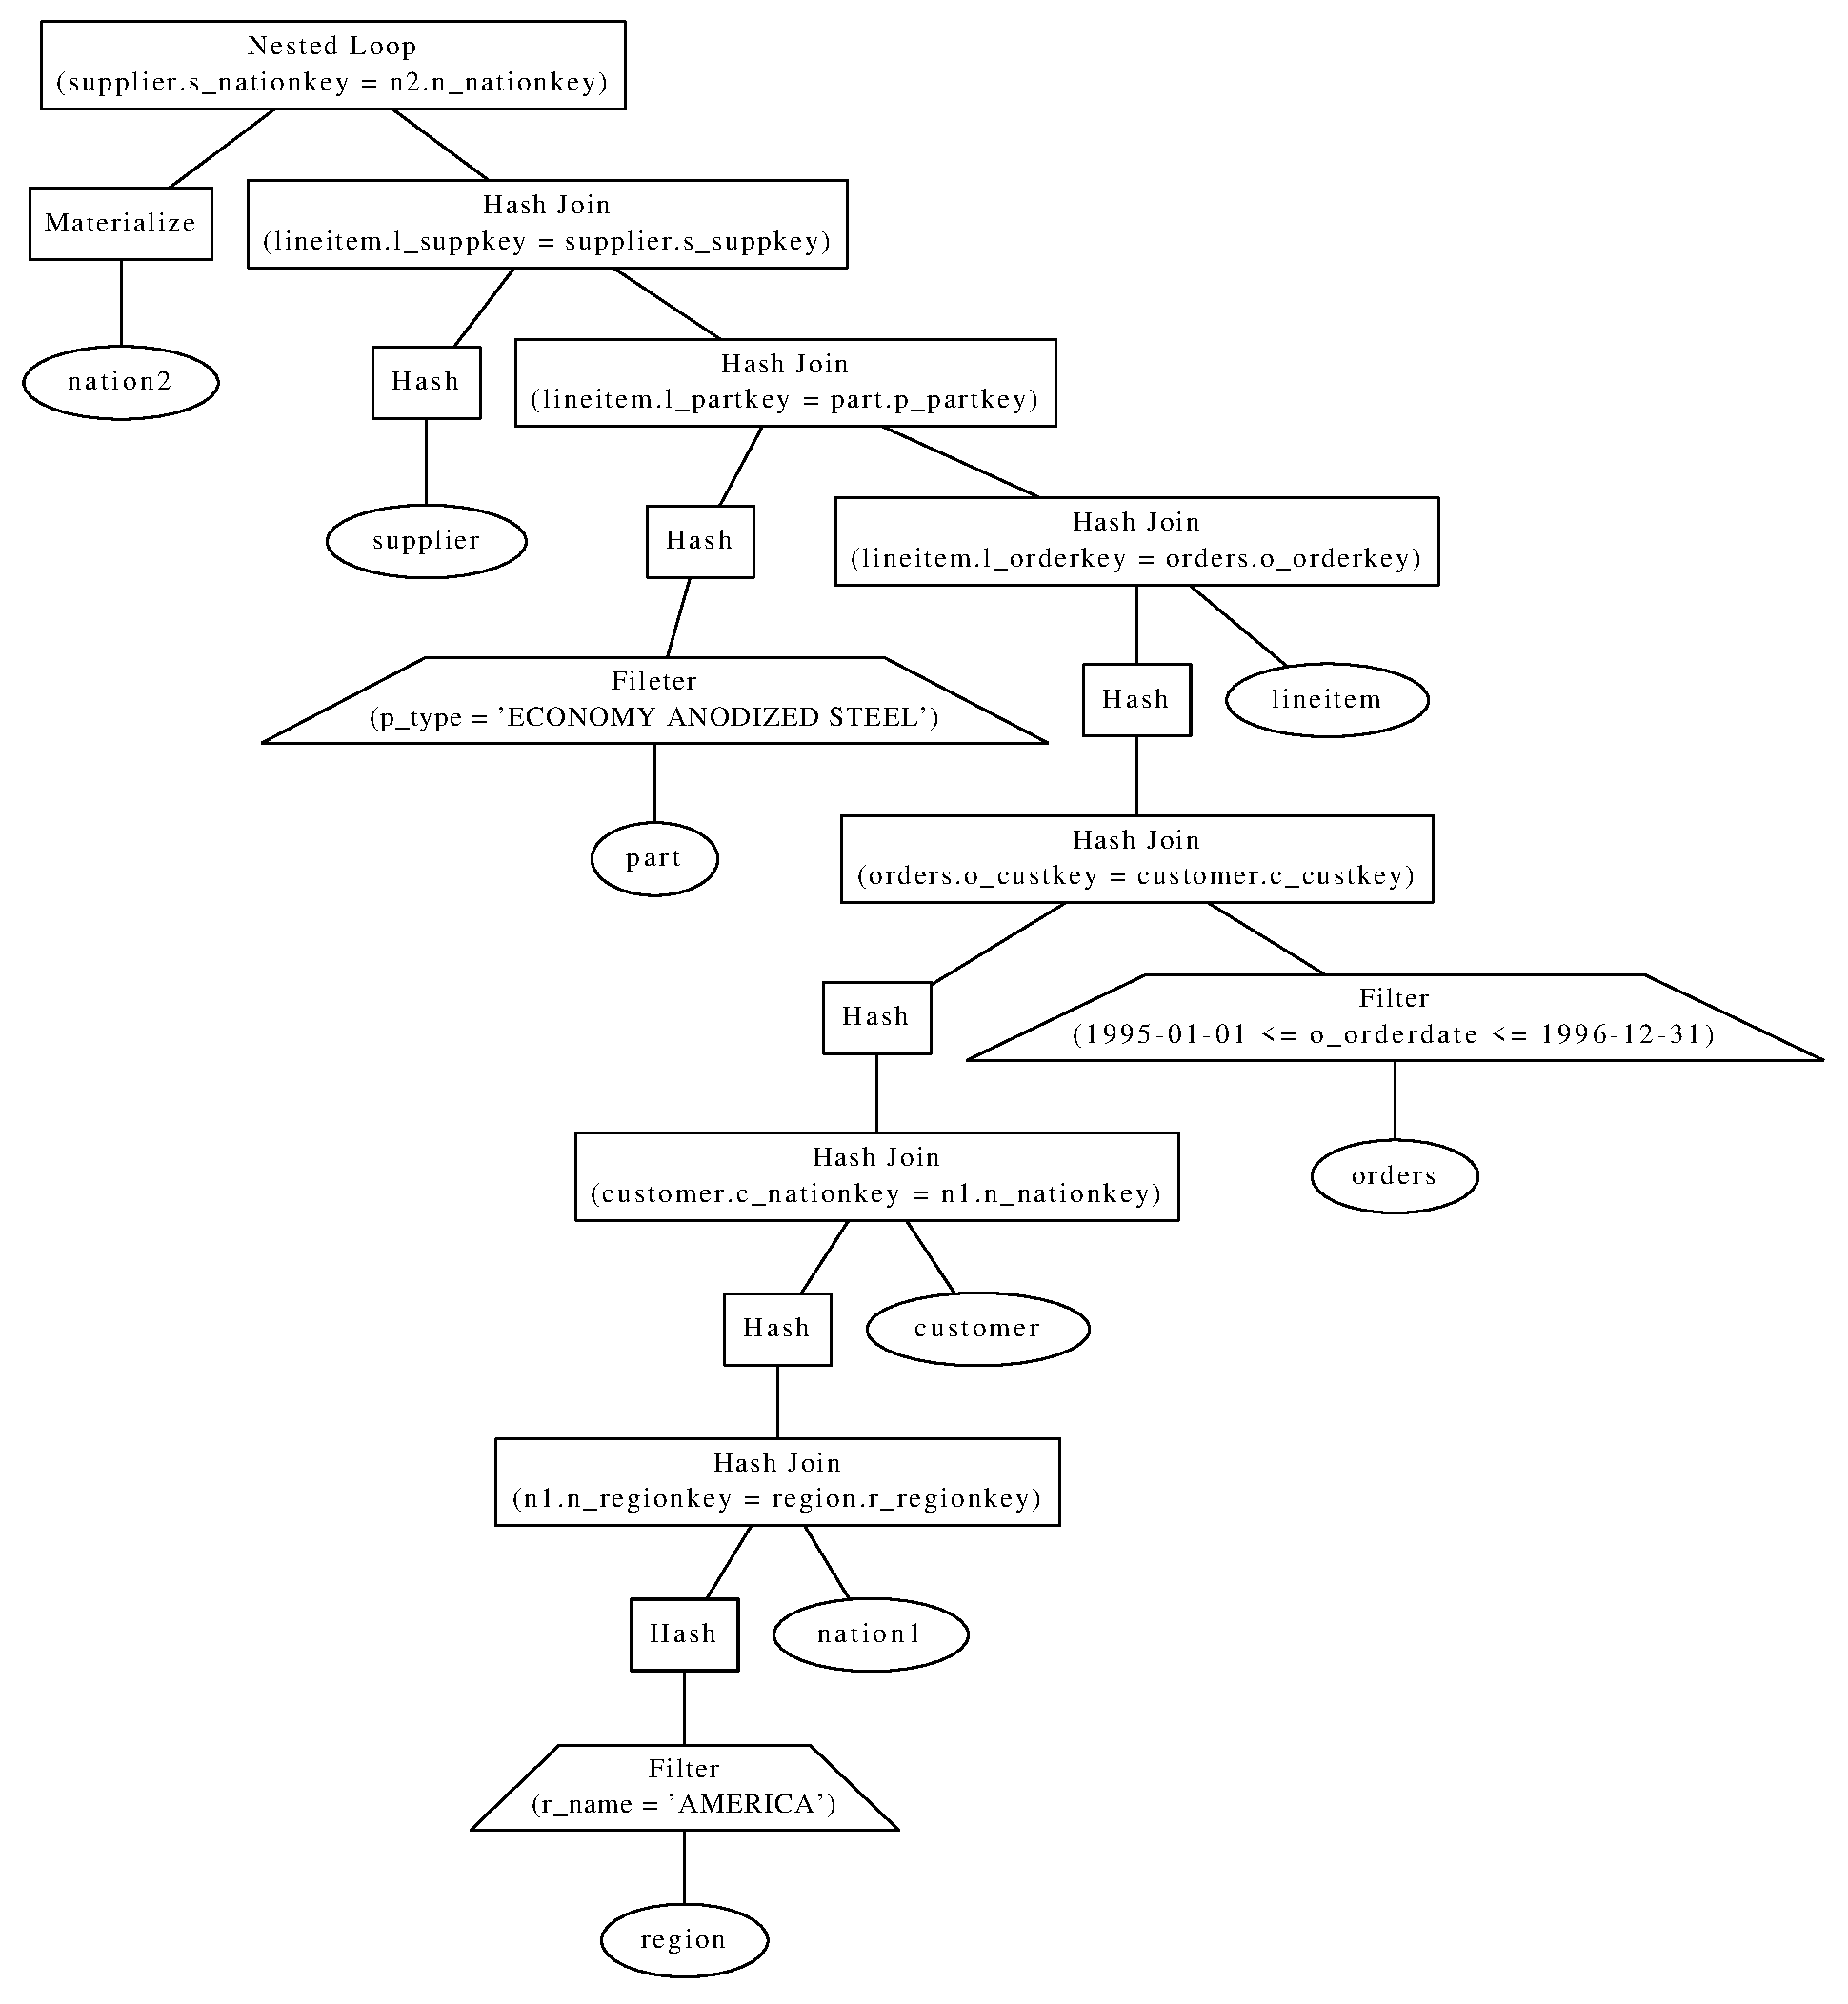
\includegraphics[width=170mm]{query8.eps}
 \end{center}
 \caption{Query 8 execution plan}
 \label{fig:query8}
\end{figure}

\clearpage
\subsection{結果}
\begin{figure}[thbp]
 \begin{center}
  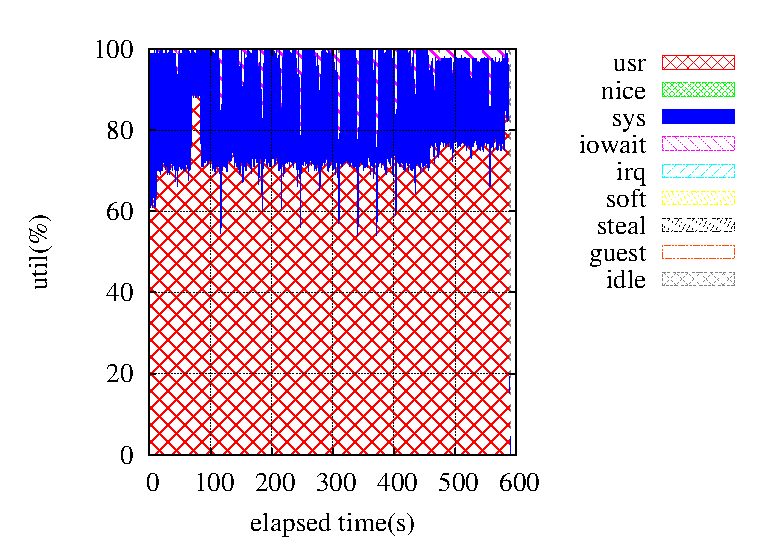
\includegraphics[width=110mm]{8corecore1.eps}
 \end{center}
 \caption{cpu utilization}
 \label{fig:8cpu}
\end{figure}

\begin{figure}[thbp]
 \setlength{\subfigwidth}{.5\linewidth}
 \addtolength{\subfigwidth}{-.5\subfigcolsep}
 \begin{minipage}[b]{\subfigwidth}
  \subfigure[IOPS]{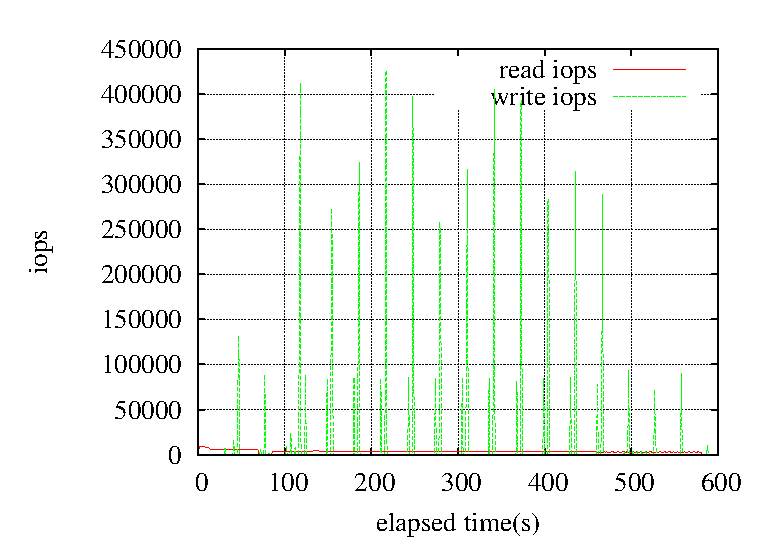
\includegraphics[width=75mm]{8coreiops.eps}
  \label{fig:8coreiops}}
 \end{minipage}
  \begin{minipage}[b]{\subfigwidth}
    \subfigure[MBPS]{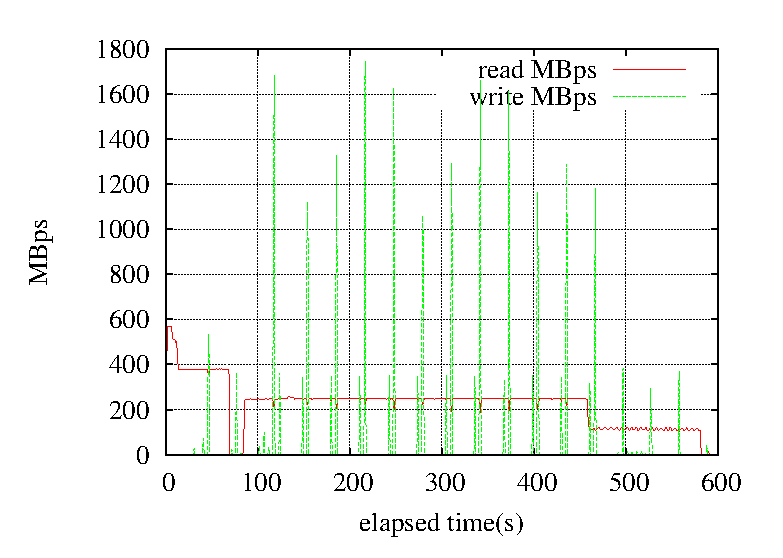
\includegraphics[width=75mm]{8corembps.eps}
   \label{fig:8corembps}}
  \end{minipage}
  \caption{IO spec}
  \label{fig:8core}
\end{figure}

\end{document}
